\chapter{ANÁLISIS DE RESULTADOS}
\section{Resultados}

El presente capítulo tiene como finalidad analizar los resultados obtenidos a partir de la implementación de modelos predictivos aplicados a las ventas de la empresa \textbf{Market Dona}, enfocándose principalmente en la categoría de frutas. El propósito del estudio no solo fue obtener predicciones precisas de ventas, sino contribuir a la solución de uno de los principales problemas identificados en la empresa: el \textbf{sobrestock y la falta de stock de productos}.

Actualmente, Market Dona enfrenta dificultades relacionadas con la gestión de inventario debido a compras realizadas sin una estimación precisa de la demanda. Esta situación ocasiona dos escenarios negativos para la empresa. Por un lado, el exceso de productos genera sobrestock, incrementando pérdidas económicas por deterioro, especialmente en productos perecibles como las frutas. Por otro lado, una compra insuficiente provoca quiebres de stock, ocasionando pérdida de ventas y disminución de satisfacción en los clientes.

Frente a esta problemática, la investigación propone el uso de modelos predictivos como herramienta de apoyo para la toma de decisiones de compra. La finalidad es alcanzar un equilibrio adecuado entre la cantidad de productos adquiridos y la demanda real esperada. Para ello, se utilizó la predicción de ventas como base para elaborar un presupuesto de compra más preciso, permitiendo a Market Dona adquirir cantidades más cercanas a las necesidades reales del negocio.

De acuerdo con los resultados obtenidos, el modelo seleccionado como mejor alternativa fue \textbf{Linear Regression}, debido a que presentó los mejores indicadores de desempeño entre los modelos evaluados. Los resultados obtenidos fueron un \textbf{MAE de 399.57}, un \textbf{MSE de 279,381.62}, un \textbf{RMSE de 528.57} y un \textbf{$R^{2}$ de 0.744}.

El valor de \textbf{$R^{2} = 0.744$} indica que el modelo logra explicar aproximadamente el \textbf{74.4\% del comportamiento de las ventas}, lo que demuestra una capacidad adecuada para representar la tendencia de demanda en la categoría fruta. Esto es importante para Market Dona, ya que permite contar con estimaciones más confiables al momento de planificar las compras.

\begin{figure}
	\centering
	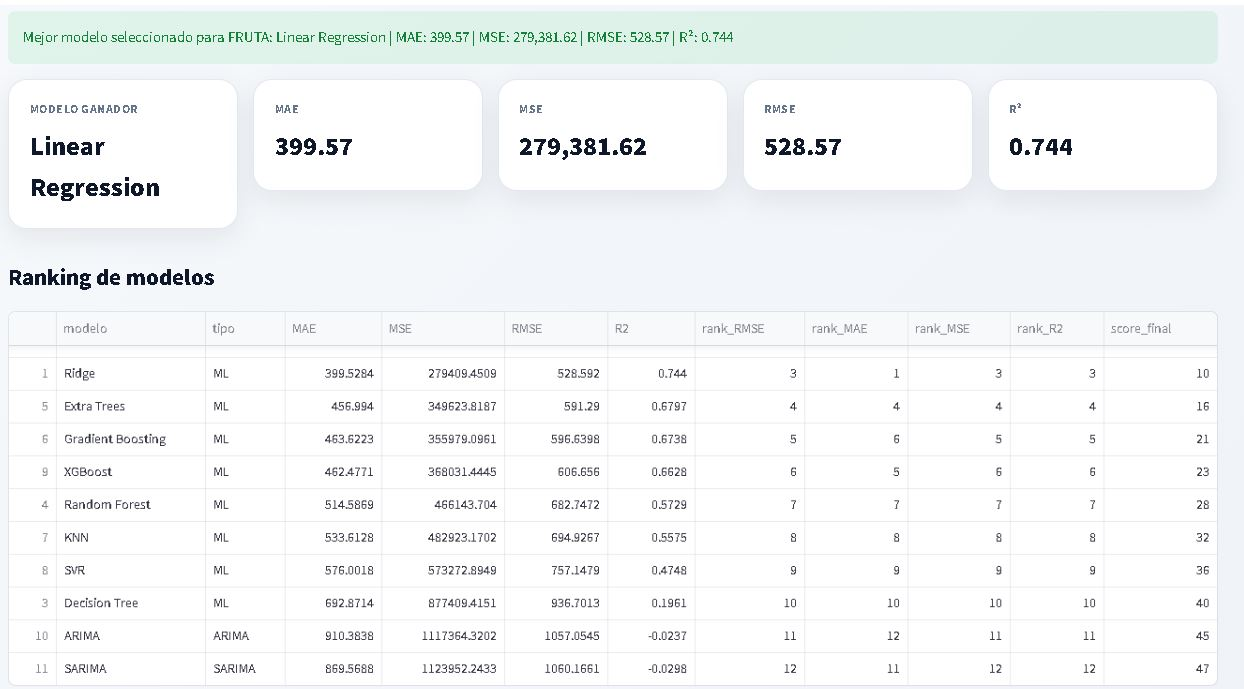
\includegraphics[width=0.8\textwidth]{4/Desa_ima/Propuestasol1.JPG}
	\caption{Gráfico de ventas reales vs predicción}
	\label{fig:real_vs_pred}
\end{figure}


Asimismo, el \textbf{MAE de 399.57} refleja que el margen promedio de error del modelo es relativamente bajo en comparación con el volumen general de ventas. Esto significa que las predicciones obtenidas pueden utilizarse como referencia válida para definir presupuestos de abastecimiento y reducir decisiones basadas únicamente en experiencia empírica o intuición.

En el gráfico de ventas reales versus predicción se observa que las predicciones mantienen un comportamiento cercano a las ventas reales durante gran parte del periodo evaluado. Aunque existen algunas diferencias en momentos de alta variabilidad, el modelo logra seguir la tendencia general del mercado. Este comportamiento resulta favorable para la empresa, debido a que permite anticipar cambios en la demanda y ajustar las compras de manera más eficiente.

Los resultados también evidencian que los modelos de Machine Learning obtuvieron un mejor desempeño que los modelos tradicionales de series temporales, como ARIMA y SARIMA. Estos últimos presentaron errores más elevados y valores negativos de $R^{2}$, lo cual indica una menor capacidad para representar el comportamiento real de las ventas. Esto sugiere que las ventas de Market Dona dependen no solo del tiempo, sino también de múltiples factores dinámicos que los modelos de aprendizaje automático pueden captar de mejor manera.

\begin{figure}
	\centering
	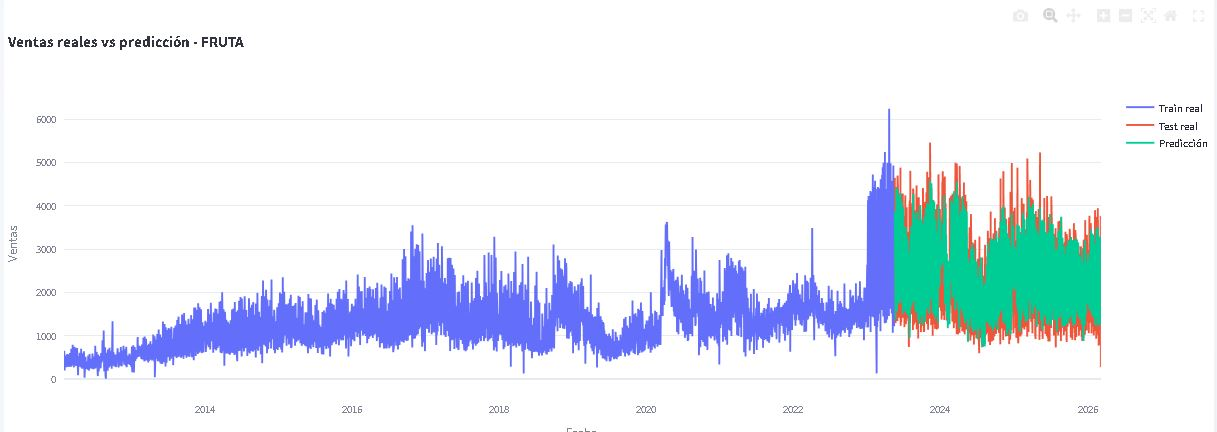
\includegraphics[width=0.9\textwidth]{4/Desa_ima/Propuestasol2.JPG}
	\caption{Gráfico de ventas reales vs predicción}
	\label{fig:real_vs_pred}
\end{figure}


La implementación de este sistema predictivo representa una mejora significativa para la gestión comercial de Market Dona. Mediante el uso de presupuestos basados en predicción de ventas, la empresa puede planificar mejor sus compras y mantener un equilibrio más adecuado entre oferta y demanda. Esto permite:

\begin{itemize}
    \item Reducir pérdidas ocasionadas por productos vencidos o deteriorados.
    \item Disminuir costos de almacenamiento innecesario.
    \item Evitar quiebres de stock y pérdida de clientes.
    \item Mejorar la disponibilidad de productos.
    \item Optimizar el uso del capital destinado a compras.
    \item Fortalecer la toma de decisiones basada en datos.
\end{itemize}

En términos prácticos, la predicción de ventas se convierte en una herramienta de apoyo para determinar cuánto comprar en cada periodo, evitando tanto compras excesivas como compras insuficientes. De esta manera, la empresa puede alcanzar un equilibrio de inventario que contribuya a mejorar su rentabilidad y eficiencia operativa.

Finalmente, los resultados demuestran que la aplicación de modelos predictivos en Market Dona puede contribuir significativamente a mejorar la gestión de inventario y el proceso de abastecimiento. El uso del modelo Linear Regression permitió obtener predicciones suficientemente precisas para apoyar la elaboración de presupuestos de compra, ayudando a reducir el sobrestock y minimizar la falta de productos, generando así un impacto positivo en las ventas y en la administración general de la empresa.



% A continuación de muestran los resultados obtenidos a partir de la metodología seguida. Estos resultados abarcan diferentes modelos de predicción como LSTM, Prophet, SVR, ARIMA, Linear Regression, Random Forest, Decision Tree, XGBoost. 

% \begin{enumerate}
% 	\item \textbf{LSTM (Long Short-Term Memory)}
% 		\begin{itemize}
% 			\item \textbf{Uso:} Redes neuronales recurrentes diseñadas para analizar datos secuenciales, como series temporales.
% 			\item \textbf{Escenarios: } Aplicaciones incluyen pronósticos de series temporales, procesamiento de lenguaje natural (NLP), y reconocimiento de voz.
% 			\item \textbf{Predictor: } Destacado por su capacidad para modelar patrones complejos y dependencias a largo plazo en datos de ventas.
% 		\end{itemize}
		
% 	\item \textbf{Prophet}
% 	\begin{itemize}
% 		\item \textbf{Uso: } Modelo de series temporales desarrollado por Facebook para prever datos con estacionalidad y tendencias cambiantes.
% 		\item \textbf{Escenarios: } Utilizado en pronósticos de ventas, gestión de inventarios y planificación de recursos.
% 		\item \textbf{Predictor: } Eficiente para capturar variaciones estacionales y cambios de tendencia en datos de ventas.
% 	\end{itemize}
	
% 	\item \textbf{SVR (Support Vector Regression)}
% 	\begin{itemize}
% 		\item \textbf{Uso: } Algoritmo de aprendizaje supervisado que encuentra un hiperplano óptimo en un espacio dimensional alto para la regresión.
% 		\item \textbf{Escenarios: } Aplicado en predicción de series temporales, análisis financiero y clasificación.
% 		\item \textbf{Predictor: } Efectivo cuando hay una separación clara entre los datos de ventas y se necesita evitar el sobreajuste.
% 	\end{itemize}
	
% 	\item \textbf{ARIMA (AutoRegressive Integrated Moving Average) }
% 	\begin{itemize}
% 		\item \textbf{Uso: } Modelo estadístico para analizar y pronosticar series temporales.
% 		\item \textbf{Escenarios: } Usado en pronóstico de demanda, análisis económico y finanzas.
% 		\item \textbf{Predictor: } Adecuado para datos de ventas con patrones estacionarios lineales o estacionales.
% 	\end{itemize}
	
% 	\item \textbf{Linear Regression}
% 	\begin{itemize}
% 		\item \textbf{Uso: } Modelo básico de regresión que asume una relación lineal entre variables.
% 		\item \textbf{Escenarios: } Aplicado en predicción de precios, análisis de mercado y evaluación de impacto.
% 		\item \textbf{Predictor: } Simple y rápido, útil cuando se requiere una interpretación clara de las relaciones entre variables.
% 	\end{itemize}
	
% 	\item \textbf{Random Forest}
% 	\begin{itemize}
% 		\item \textbf{Uso: } Método de aprendizaje en conjunto que combina múltiples árboles de decisión para mejorar la precisión.
% 		\item \textbf{Escenarios: } Utilizado en clasificación y regresión, detección de anomalías y análisis predictivo de marketing.
% 		\item \textbf{Predictor: } Eficiente para grandes conjuntos de datos con muchas variables, capturando relaciones no lineales.
% 	\end{itemize}
	
% 	\item \textbf{Decision Tree}
% 	\begin{itemize}
% 		\item \textbf{Uso: } Modelo que divide el conjunto de datos en subconjuntos más pequeños según características específicas.
% 		\item \textbf{Escenarios: } Aplicaciones en análisis de riesgos, diagnósticos médicos y segmentación de mercado.
% 		\item \textbf{Predictor: } Fácil de interpretar y visualizar, adecuado para datos estructurados y no estructurados.
% 	\end{itemize}
	
% 	\item \textbf{XGBoost (Extreme Gradient Boosting)}
% 	\begin{itemize}
% 		\item \textbf{Uso: } Algoritmo de aprendizaje en conjunto que utiliza árboles de decisión potenciados con gradientes.
% 		\item \textbf{Escenarios: } Utilizado en competiciones de Kaggle, pronóstico de series temporales, clasificación y regresión.
% 		\item \textbf{Predictor: } Potente para mejorar la precisión en grandes conjuntos de datos, especialmente en problemas complejos de predicción de ventas.
% 	\end{itemize}	
% \end{enumerate}


% %%%CAMBIO
% En la investigaación sobre la predicción de ventas en Market Donna, se evaluó varios modelos para determinar su eficacia. Tras analizar métricas como MSE, RMSE, R\textsuperscript{2} y MAPE, se encontró que el modelo de Regresión Lineal destacó como el mejor predictor entre los comparados. Con un MSE de 0.282840 y un RMSE de 0.531821, Regresión Lineal demostró una precisión superior en las predicciones en comparación con modelos como Prophet, SVR, ARIMA, LSTM, Random Forest, Decision Tree y XGBoost, los cuales mostraron métricas menos favorables. Este resultado destacó la capacidad de la regresion lineal para capturar patrones complejos en las series temporales de ventas de Market Donna, resaltando su relevancia en aplicaciones donde la exactitud en la predicción era crucial para la toma de decisiones estratégicas y operativas.


% %%CAMBIO
% \begin{table}[H]
% 	\centering
% 	\caption{Comparación de metricas}
% 	\begin{tabular}{lcccc}
% 		\hline
% 		& MSE      & RMSE     & R\textsuperscript{2}  & MAPE       \\ \hline
% 		LSTM                    & 0.253145 & 0.503135 & 0.311354 & 1.901903   \\
% 		Prophet                 & 0.347766 & 0.589717 & 0.053949 & 1.680879   \\
% 		SVR                     & 0.261895 & 0.511757 & 0.287550 & 1.435059   \\
% 		ARIMA                   & 0.366476 & 0.605372 & 0.003053 & 0.999000   \\
% 		Linear Regression       & 0.282840 & 0.531827 & 0.230572 & 1.940515   \\
% 		Random Forest           & 0.312075 & 0.558636 & 0.151043 & 3.434788   \\
% 		Decision Tree           & 0.350198 & 0.591775 & 0.047334 & 4.422758   \\
% 		XGBoost                 & 0.360486 & 0.600405 & 0.019348 & 2.744646  \\ \hline
% 	\end{tabular}
% 	\newline
% 	\newline \textit{Fuente: Elaboración propia}
% 	\label{table:models_comparison}
% \end{table}



%\section{Y}
%
%Nisi porta lorem mollis aliquam ut porttitor leo. Aenean pharetra magna ac placerat vestibulum. Est placerat in egestas erat imperdiet sed euismod. Velit euismod in pellentesque massa placerat. Enim praesent elementum facilisis leo vel fringilla. Ante in nibh mauris cursus mattis molestie a iaculis. Erat pellentesque adipiscing commodo elit at imperdiet dui accumsan sit. Porttitor lacus luctus accumsan tortor posuere ac ut. Tortor at auctor urna nunc id. A iaculis at erat pellentesque adipiscing commodo elit. 
%
%
%\section{Z}
%
%Nisi porta lorem mollis aliquam ut porttitor leo. Aenean pharetra magna ac placerat vestibulum. Est placerat in egestas erat imperdiet sed euismod. Velit euismod in pellentesque massa placerat. Enim praesent elementum facilisis leo vel fringilla. Ante in nibh mauris cursus mattis molestie a iaculis. Erat pellentesque adipiscing commodo elit at imperdiet dui accumsan sit. Porttitor lacus luctus accumsan tortor posuere ac ut. Tortor at auctor urna nunc id. A iaculis at erat pellentesque adipiscing commodo elit.
